\documentclass{article}
\usepackage{amsmath}  % 数学符号包
\usepackage{amssymb}  % 更多数学符号
\usepackage{enumitem} % 列表样式
\usepackage{fancyhdr} % 页眉设置
\usepackage{geometry} % 页面设置
\usepackage[UTF8]{ctex}
\usepackage{caption}
\usepackage{bm}
\usepackage{amsthm}
\usepackage{graphicx}
\usepackage{tabularx}
\usepackage{booktabs}
\usepackage{xcolor}
\usepackage{float}
\usepackage{minted}
\everymath{\displaystyle}  % 让所有数学模式都使用 \displaystyle
\newcommand{\lb}{\left\llbracket}
\newcommand{\rb}{\right\rrbracket}
\newcommand{\np}{\noindent\par}

\definecolor{mybgcolor}{rgb}{0.95, 0.95, 0.95}  % RGB 范围在 [0, 1] 之间

\geometry{a4paper, margin=1in}


\pagestyle{fancy}
\fancyhf{}
\fancyhead[C]{电子技术与系统 -- 实验报告}
\fancyhead[R]{2025.5}


\title{电子技术与系统 -- 实验报告}
\author{Noflowerzzk}
\date{2025.5}


\begin{document}
\maketitle

\begin{tabularx}{\textwidth}{l X X}
\toprule
\textbf{分类\qquad\qquad} & \textbf{具体内容} & \textbf{完成情况} \\
\midrule
\multicolumn{3}{l}{\textbf{确保矩阵乘加速模块的功能正确(60\%)}} \\
& 阵列的整体功能(20\%):通过5组测试数据 & \textcolor{green}{完成}\\
& 乘法器功能验证(20\%):通过测试集 & \textcolor{green}{完成}\\
& 加法器功能验证(20\%):通过测试集 & \textcolor{green}{完成}\\
\midrule
\multicolumn{3}{l}{\textbf{性能指标(40\%)}} \\
& 硬件效率:所有同学的指标排序百分比 & \\
\midrule
\multicolumn{3}{l}{\textbf{加分项}} \\
& 扩展成动阵列以外的其他模块($\sim$20\%) & 无\\
& 报告中完整的逻辑功能、面积、频率分析($\sim$10\%) & 部分\\
& 对控制信号的分析、实现、验证和扩展($\sim$5\%) & 无\\
& 输入数据的处理过程分析($\sim$5\%) & 无\\
\midrule
\multicolumn{3}{l}{\textbf{减分项}} \\
& 未通过测试集 & \\
& 报告必备内容缺失 & \\
& 性能指标计算错误 & \\
\bottomrule
\end{tabularx}

\section{电路部分}

\subsection{电路结构设计}

\subsubsection{PE单元的整体设计及电路图}

\begin{figure}[H]
    \centering
    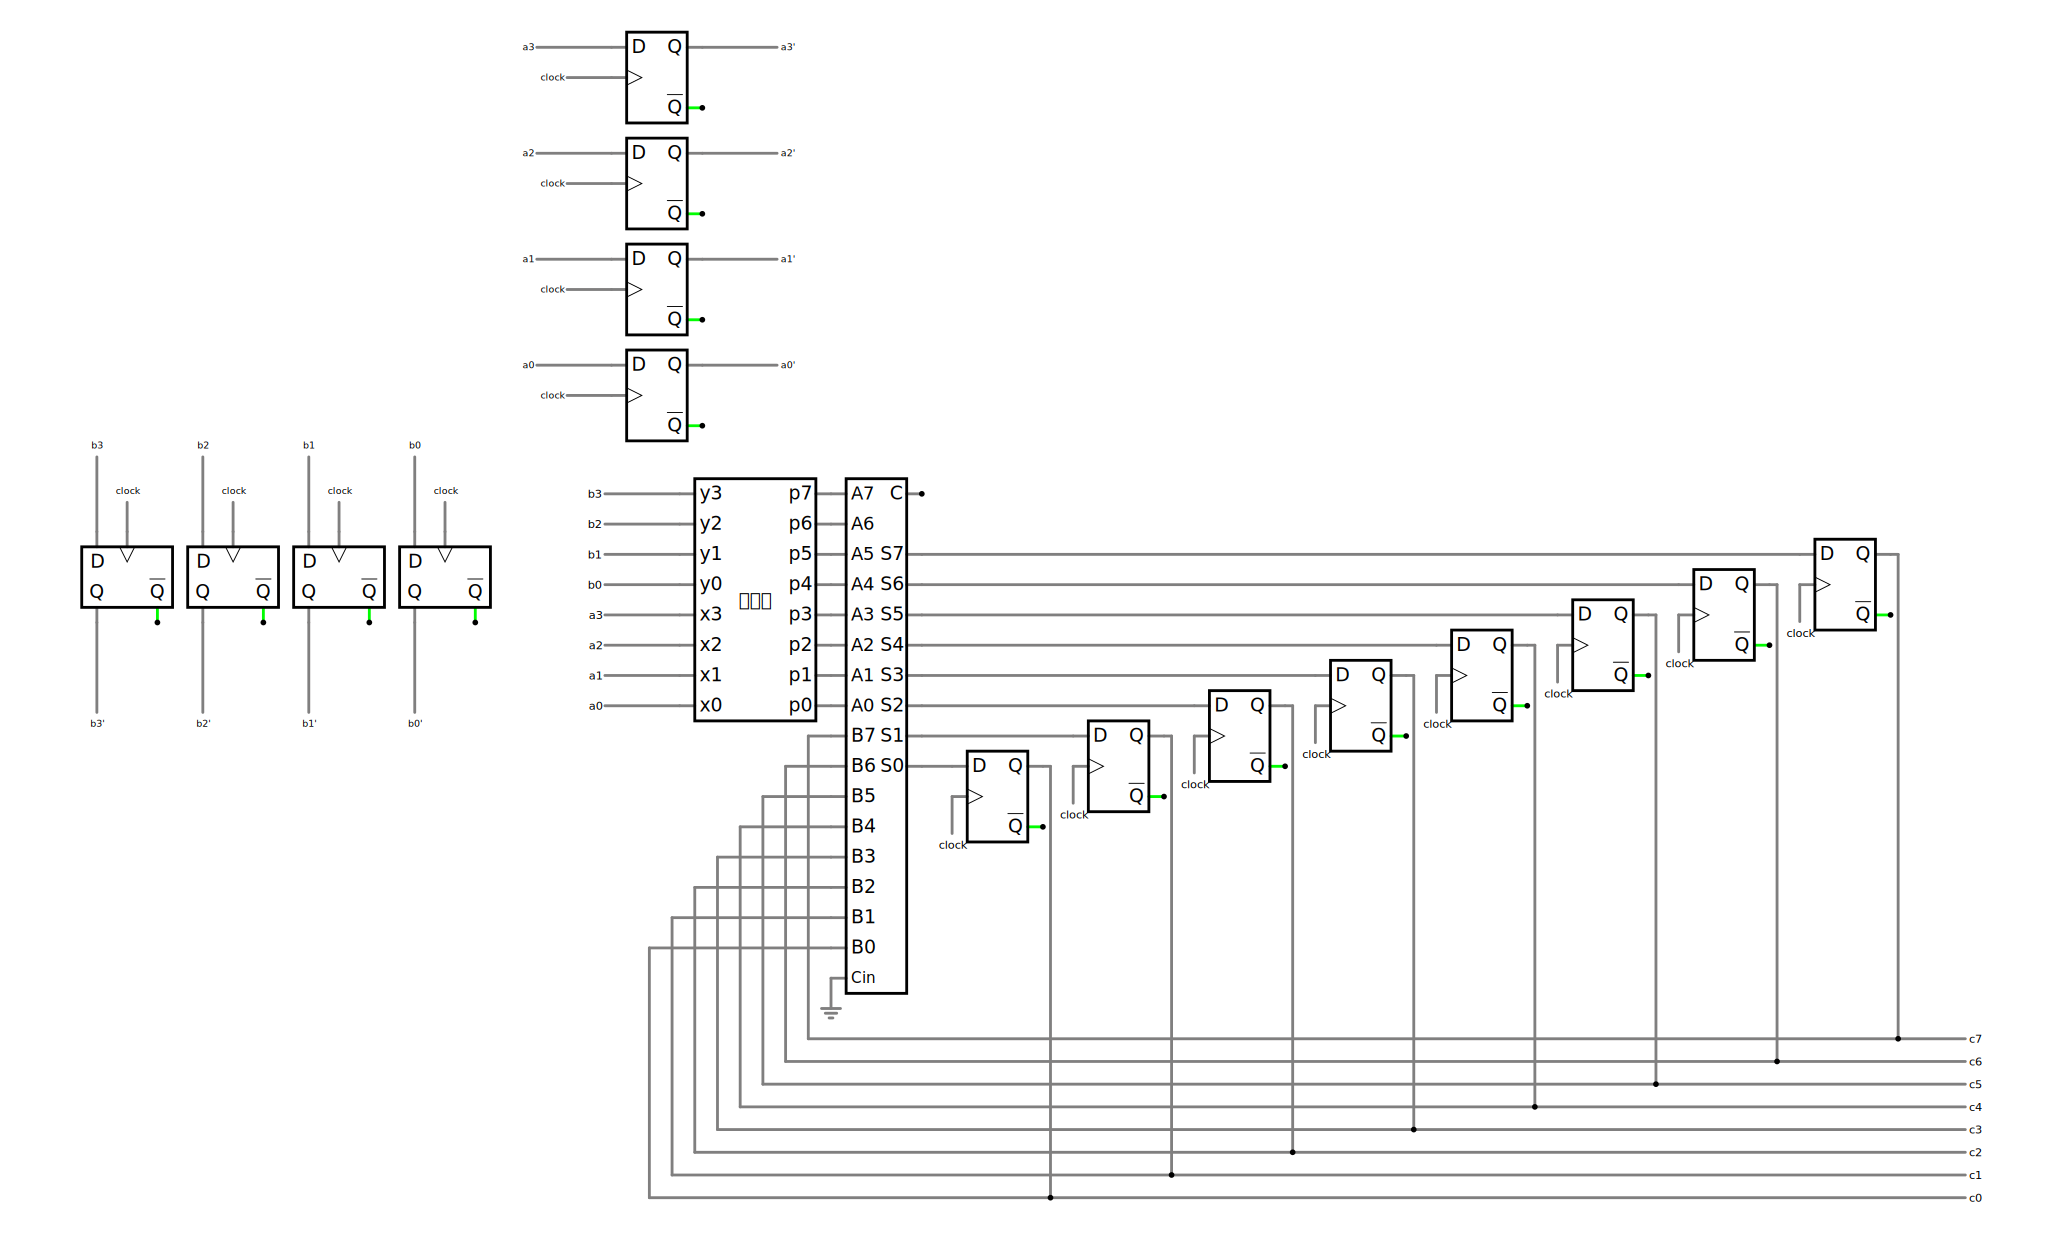
\includegraphics[width=1\textwidth]{脉动阵列.pdf}
    \caption{PE单元电路结构设计}
\end{figure}


\subsubsection{加法器电路结构设计}

此处全加器采用 Liu's 半加器组合而成

\begin{figure}[H]
    \centering
    \includegraphics[width=1\textwidth]{微信图片_20250612132911.png}
    \caption{全加器电路结构设计}
\end{figure}

\begin{figure}[H]
    \centering
    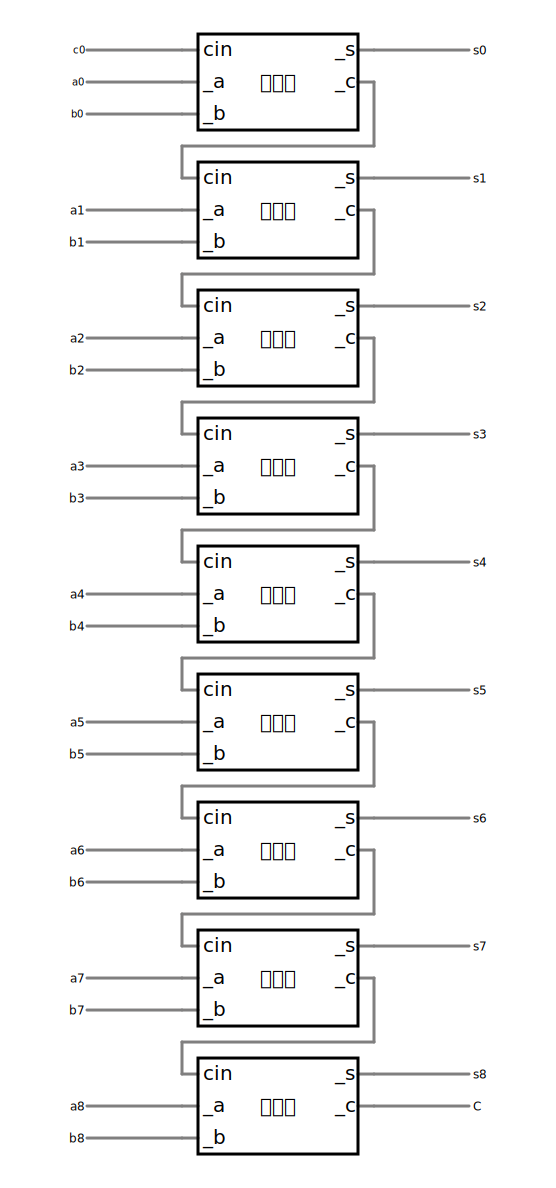
\includegraphics[width=0.5\textwidth]{8-bit加法器.pdf}
    \caption{加法器电路结构设计}
\end{figure}

\subsubsection{乘法器电路结构设计}

\begin{figure}[H]
    \centering
    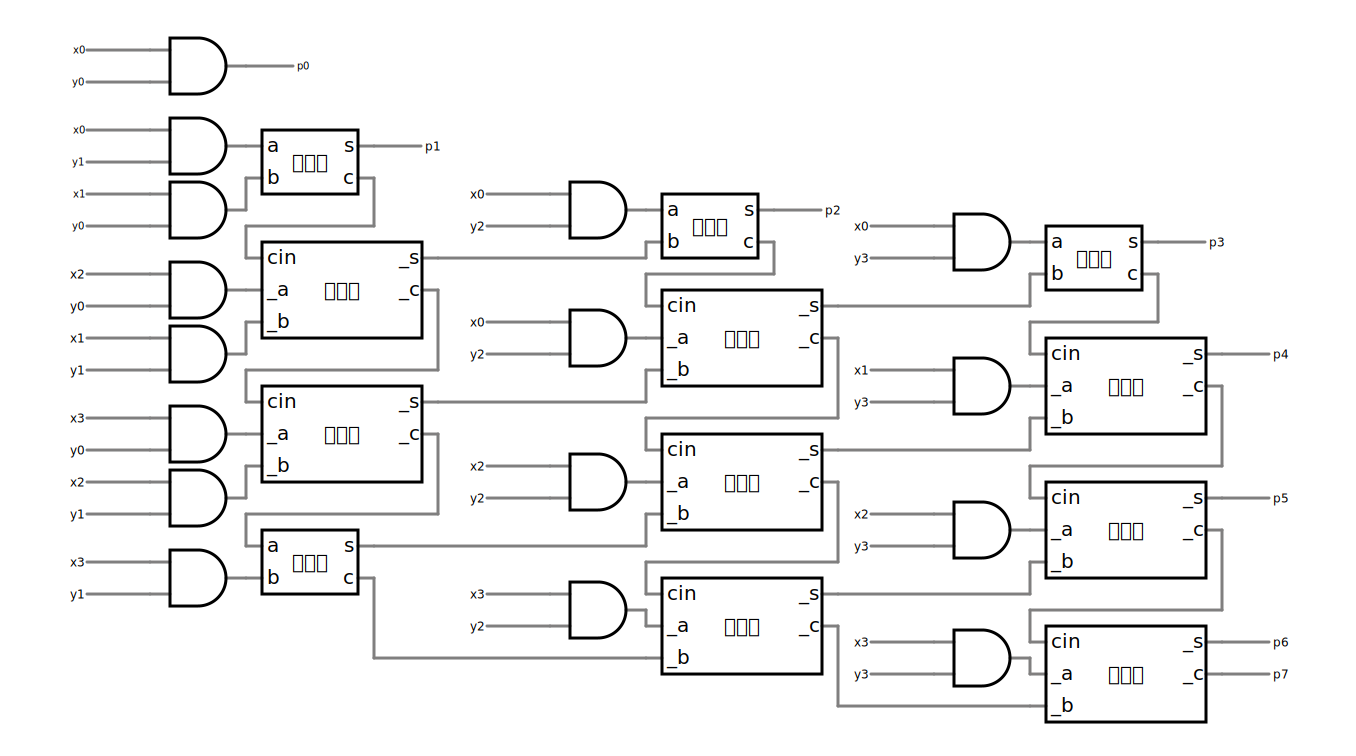
\includegraphics[width=1\textwidth]{4-bit乘法器.pdf}
    \caption{乘法器电路结构设计}
\end{figure}

\subsection{电路结构验证}

\subsubsection{PE array功能验证}

\begin{figure}[H]
    \centering
    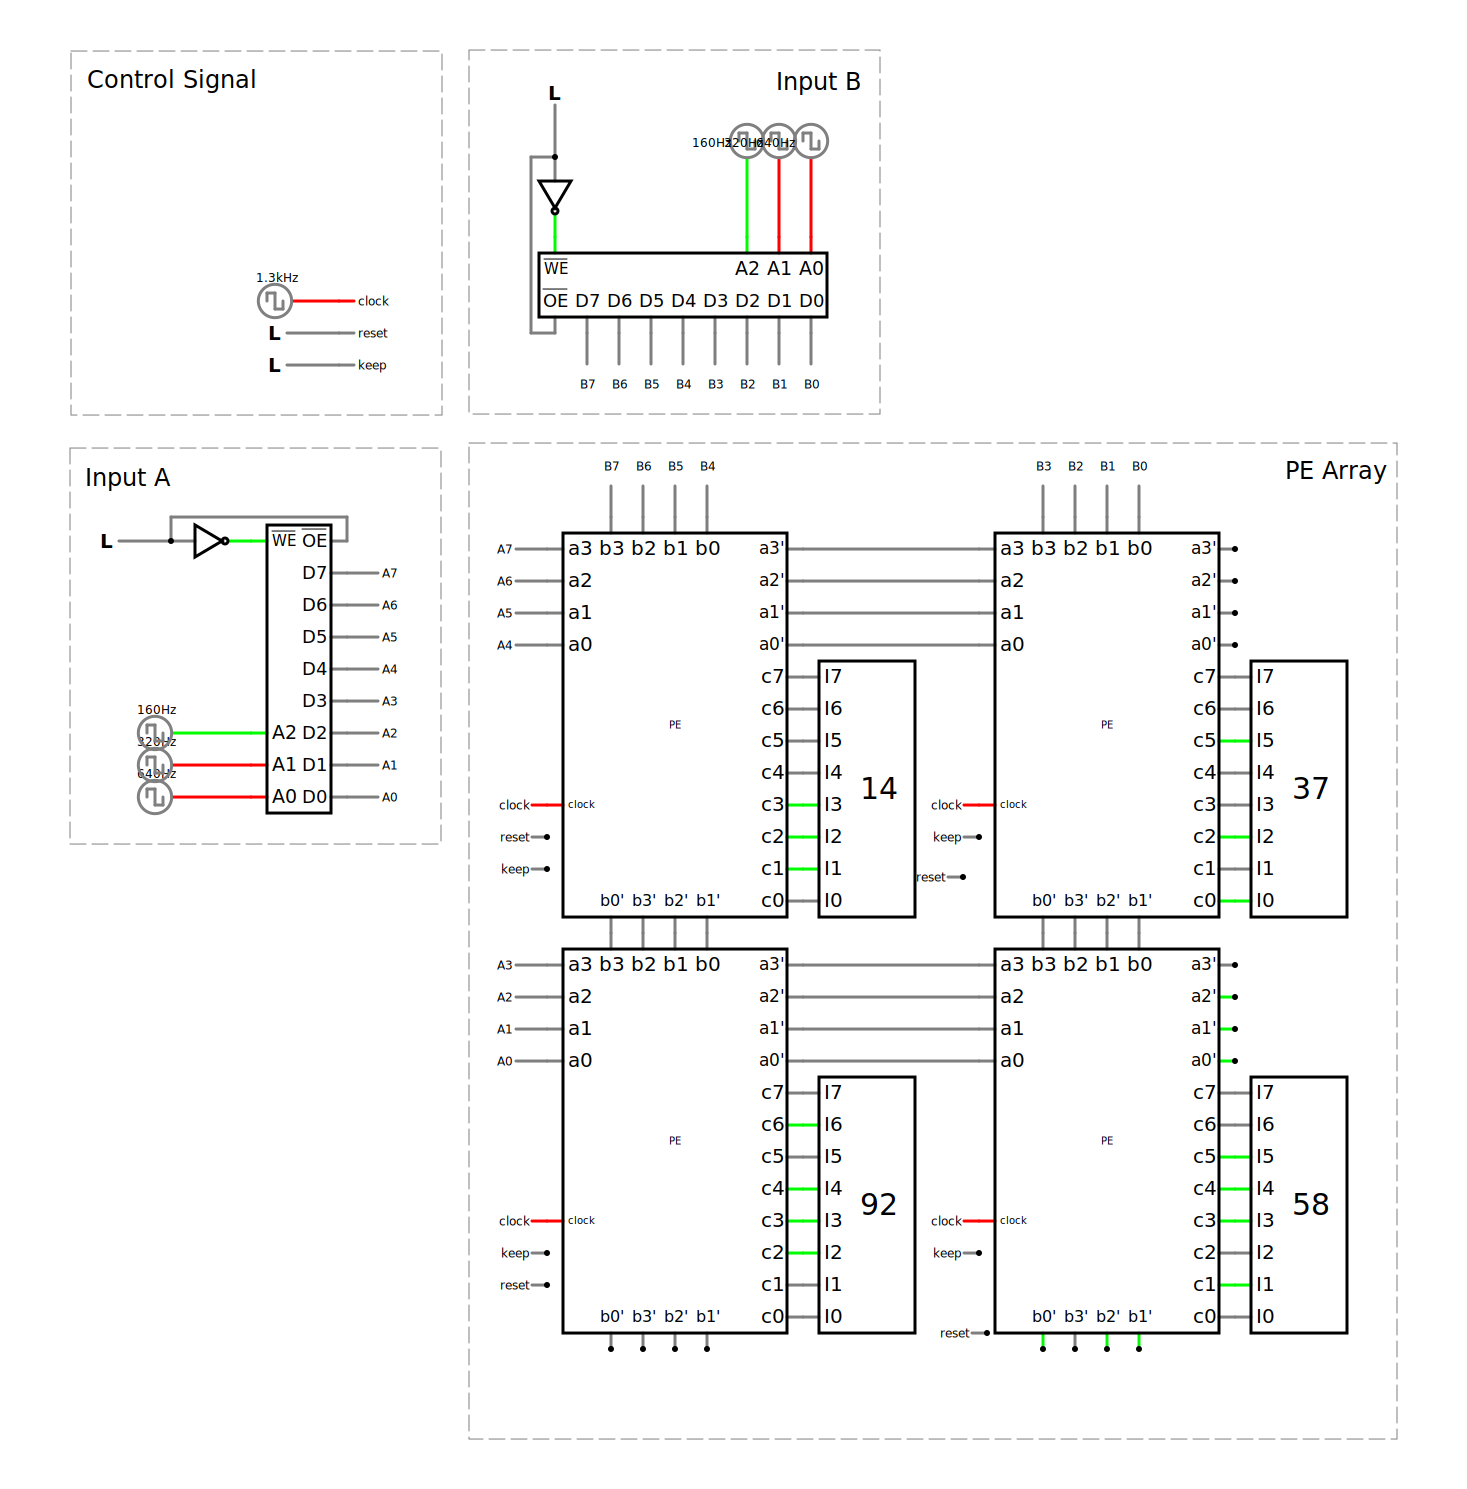
\includegraphics[width=0.7\textwidth]{PE验证_1.pdf}
    \caption{PE array功能验证}
\end{figure}

\subsubsection{乘法器功能验证}

\begin{figure}[H]
    \centering
    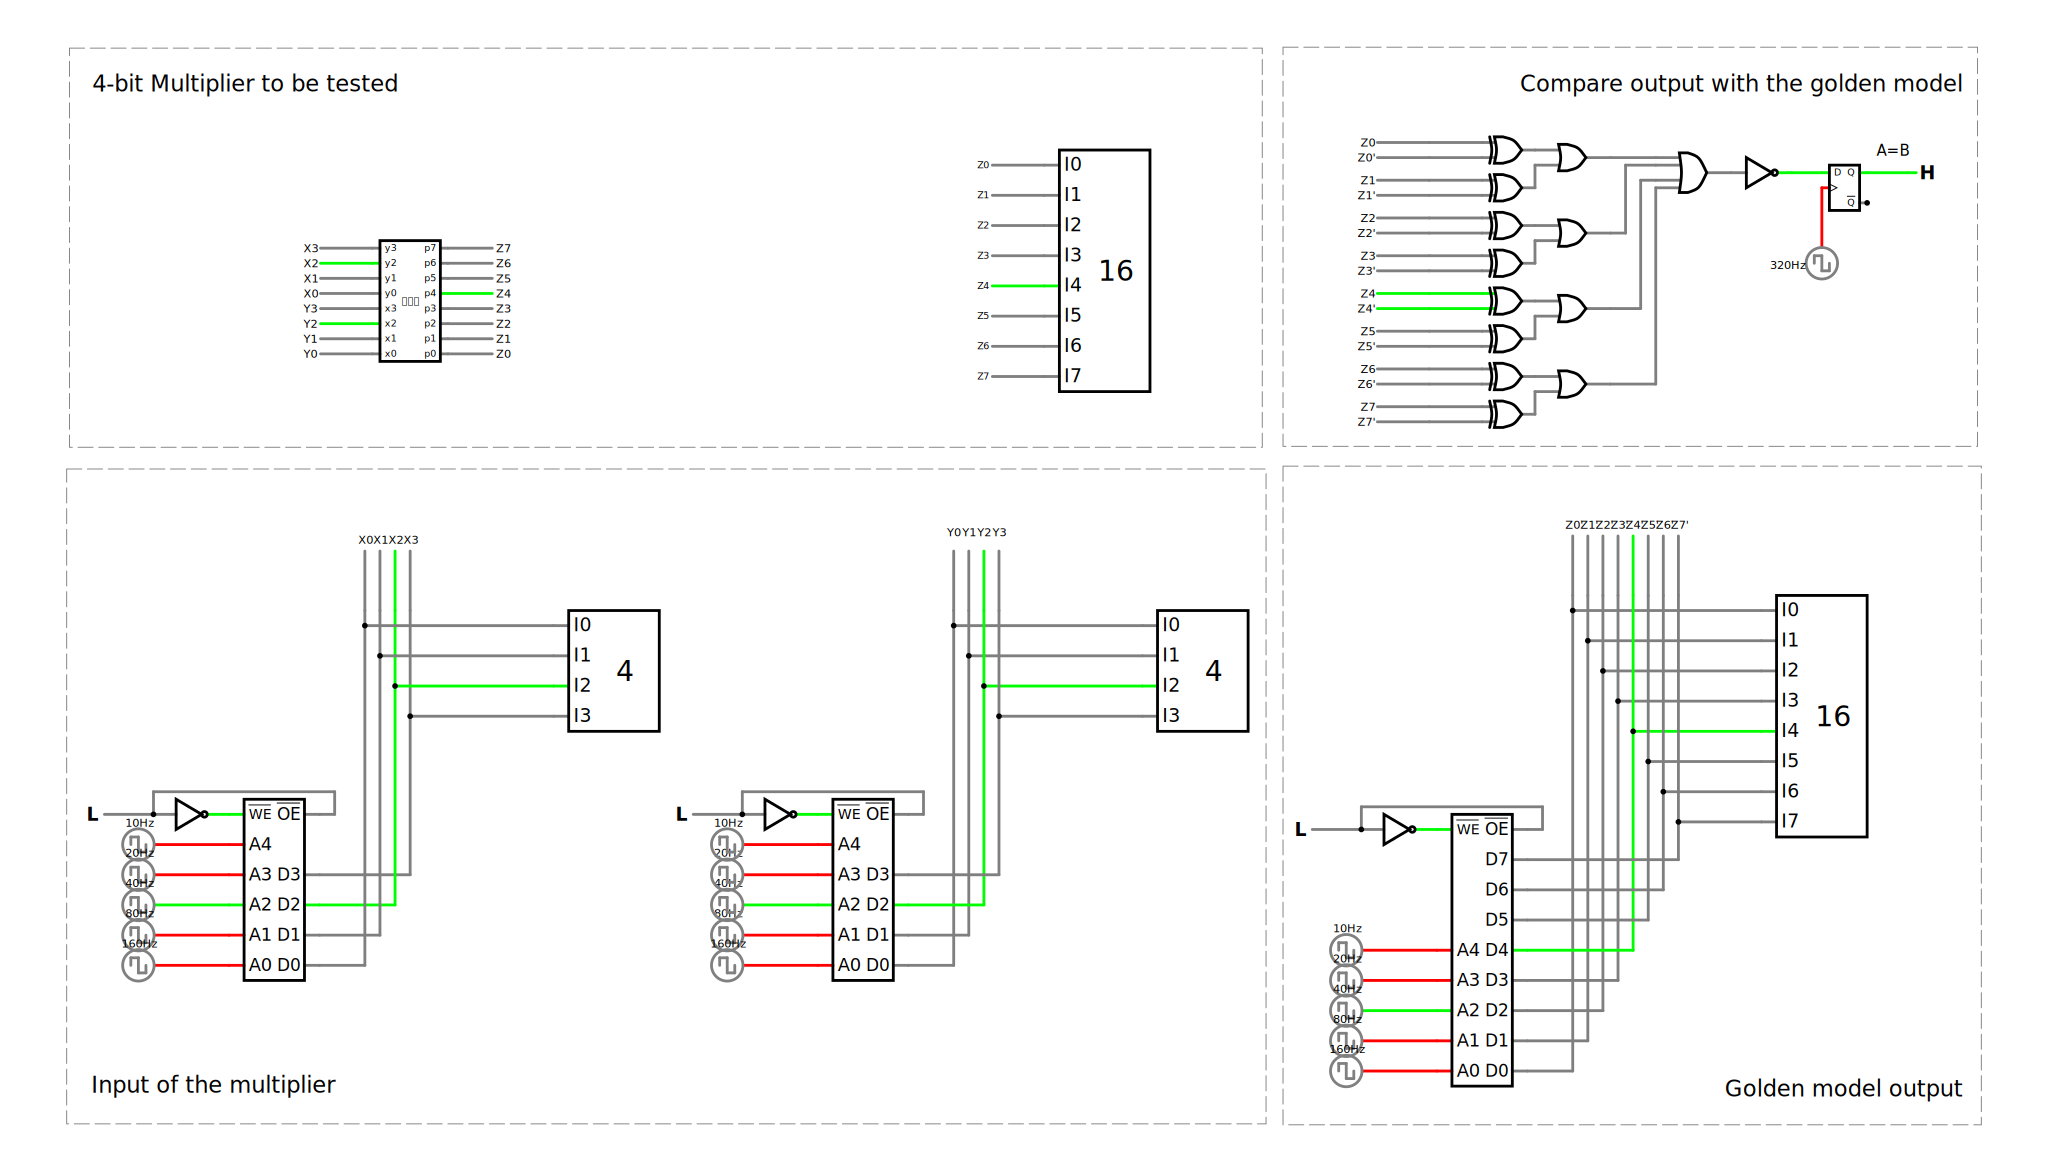
\includegraphics[width=1\textwidth]{乘法器验证.pdf}
    \caption{乘法器功能验证}
\end{figure}

\subsubsection{加法器功能验证}

\begin{figure}[H]
    \centering
    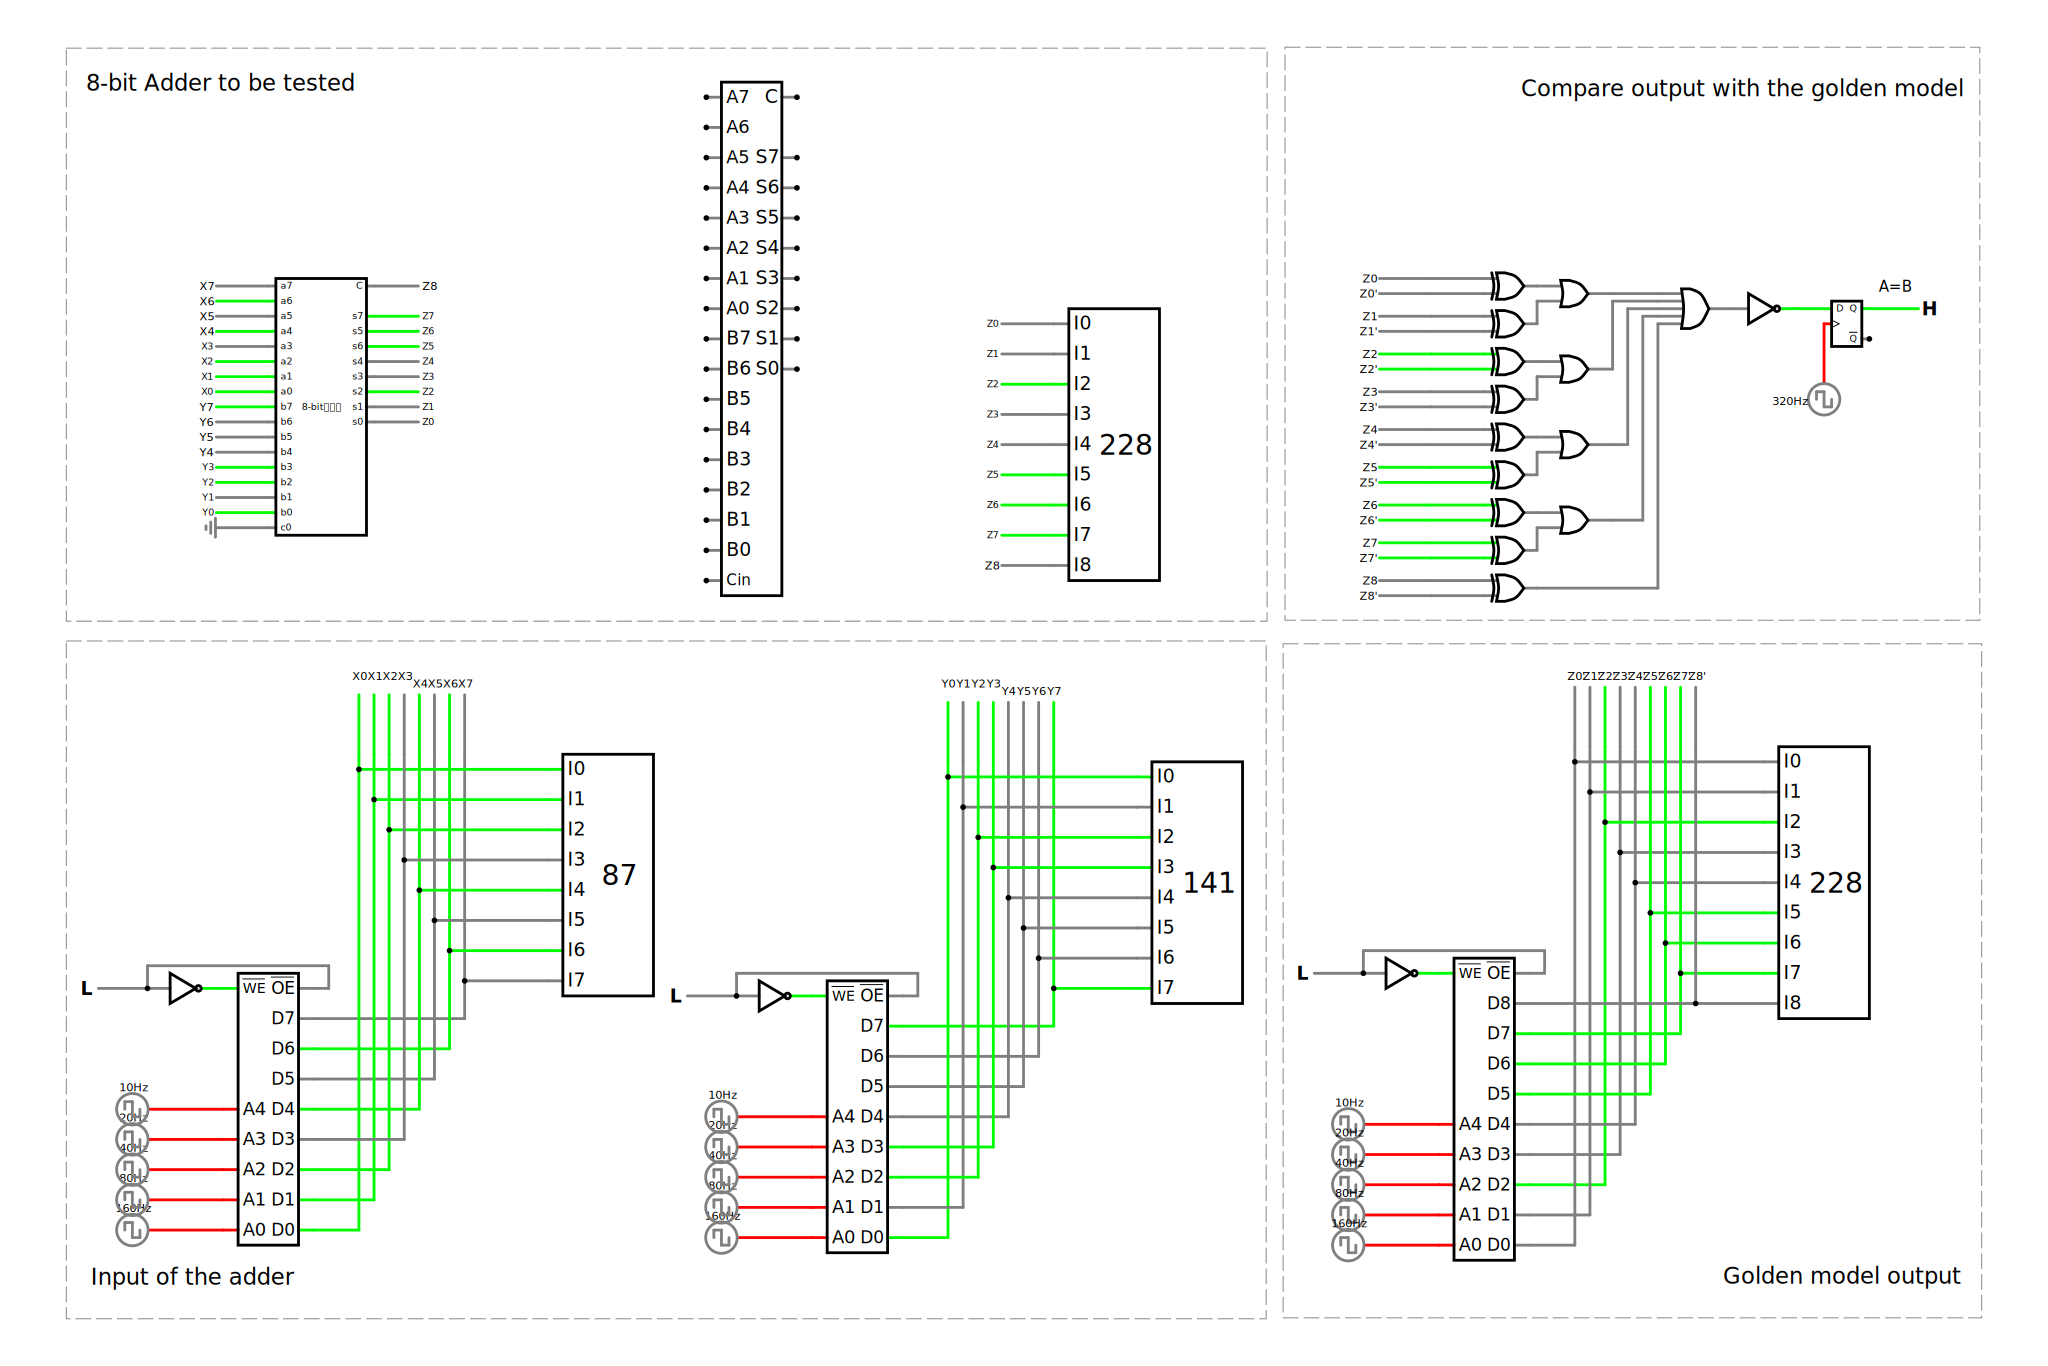
\includegraphics[width=1\textwidth]{加法器验证.pdf}
    \caption{加法器功能验证}
\end{figure}

\subsection{电路指标评估}

\subsubsection{总面积开销}

单个 PE 总面积开销为 148, 四个 PE 总面积开销为 592

\subsubsection{时序性能}

单个 PE 关键路径延迟为 6 单位,时钟周期 $T \geq 6$

\subsubsection{硬件效率计算}

单个效率为 $\frac{1}{120}$, 四个 PE 硬件效率为 $\frac{1}{480}$

\section{神经网络稀疏部分}

\subsection{模型中权重的分布}

\subsubsection{问题一解答}

共同特点:均为单峰分布,且较为集中到 0  
帮助:能大致确定稀疏度大小变化时模型精度的变化。

\subsubsection{权重分布图}

\begin{figure}[H]
    \centering
    \includegraphics[width=1\textwidth]{output.png}
    \caption{权重分布图}
\end{figure}

\subsection{基于数值大小进行细粒度剪枝}

\subsubsection{代码任务一代码}

\begin{minted}[breaklines=true, frame=single, fontsize=\small, bgcolor=mybgcolor]{python}
def fine_grained_prune(tensor: torch.Tensor, sparsity : float) -> torch.Tensor:
    """
    对单个张量进行基于数值大小的修剪
    :param tensor: torch中的Tensor, 线性层/卷积层的权重 传的是引用,有做修改
    :param sparsity: float, 目标稀疏度
        稀疏度 = 张量中0的数目 / 张量中的总元素数目 = 1 - 张量中非0的数目 / 张量中的总元素数目
    :return:
        torch.(cuda.)Tensor, 返回掩码;掩码中的True(1)代表保留相应元素;False(0)代表对相应元素执行剪枝(置为0)
    """
    sparsity = min(max(0.0, sparsity), 1.0) # 确保稀疏度在[0, 1]之间
    # 处理一些边界情况
    if sparsity == 1.0: # 稀疏度为1:全裁掉
        tensor.zero_()
        return torch.zeros_like(tensor) # 注意: 该函数返回的是掩码,全裁掉那就返回一个和原张量形状相同、全为0的张量
                                        # torch.zeros_like方法接受一个张量,返回一个和输入张量形状相同、但数值全为0的张量
    elif sparsity == 0.0: # 稀疏度为0:全保留
        return torch.ones_like(tensor) # 注意: 该函数返回的是掩码,全保留那就返回一个和原张量形状相同、全为1的张量
                                       # torch.ones_like,和zeros_like类似哦,相信你会举一反三~

    num_elements = tensor.numel() # 张量中总元素数目

    ##################### YOUR CODE STARTS HERE #####################
    # Z3dKFpREy9
    # 第一步: 对权重张量的每个元素进行打分,得到分数(重要性)张量
    importance = tensor.abs()
    # importance = torch.abs(tensor) 也行
    # 第二步: 根据分数和目标稀疏度,寻找阈值
    # threshold = importance.reshape(-1).sort(descending=False)[0][round(num_elements * sparsity) - 1]
    # threshold = importance.kthvalue()[0]   # 不指定维度的话默认在最后一个维度找 k-th, 相当于降维,返回时为最小值张量以及对应索引张量。[0] 指取值,[1] 指取索引
    threshold = importance.reshape(-1).kthvalue(round(sparsity * num_elements))[0]    # reshape 把改张量转化为一行的(自动推导) reshape(a.numel()) 也行
    # 第三步: 得到掩码
    mask = importance > threshold
    # Z3dKFpREy9
    ##################### YOUR CODE ENDS HERE #######################

    # 第四步: 将掩码作用于原权重张量
    # 注:我们这里使用了“原位操作”,即方法名后面带了个下划线`_`
    # 在Lab0.2中,我们知道多数方法会返回一个“新”张量,并不会作用到原张量上
    # 而原位操作,允许我们将计算结果,直接作用到原张量上
    tensor.mul_(mask)

    return mask # 返回掩码
\end{minted}

\subsubsection{输出结果}

\begin{figure}[H]
    \centering
    \includegraphics[width=1\textwidth]{output1.png}
    \caption{输出结果}
\end{figure}

\begin{minted}[breaklines=true, frame=single, fontsize=\small, bgcolor=mybgcolor]{output}
    * Test fine_grained_prune()
    目标稀疏度: 0.75
        剪枝前的稀疏度: 0.04
        剪枝后的稀疏度: 0.76
        掩码的稀疏度: 0.76
    * 测试通过
\end{minted}

\subsection{敏感度扫描}

\subsubsection{敏感度曲线图}

\begin{figure}[H]
    \centering
    \includegraphics[width=1\textwidth]{output3.png}
    \caption{敏感度曲线图}
\end{figure}

\subsubsection{问题二回答}
 
1. 稀疏度高,准确性低  \\
2. 不同  \\
3. 第一层最敏感,最后一层(分类器)最不敏感  \\

\subsection{指定各层的稀疏度}

\subsubsection{各层参数量图}

\begin{figure}[H]
    \centering
    \includegraphics[width=1\textwidth]{output4.png}
    \caption{各层参数量图}
\end{figure}

\subsubsection{为各层指派的稀疏度}

\begin{minted}[breaklines=true, frame=single, fontsize=\small, bgcolor=mybgcolor]{output}
    'backbone.conv0.weight': 0.5,
    'backbone.conv1.weight': 0.85,
    'backbone.conv2.weight': 0.85,
    'backbone.conv3.weight': 0.8,
    'backbone.conv4.weight': 0.8,
    'backbone.conv5.weight': 0.9,
    'backbone.conv6.weight': 0.9,
    'backbone.conv7.weight': 0.9,
    'classifier.weight': 0.9
\end{minted}

根据敏感度曲线图指派并根据后续代码微调

\subsubsection{稀疏剪枝后的权重分布图}

\begin{figure}[H]
    \centering
    \includegraphics[width=1\textwidth]{output5.png}
    \caption{稀疏剪枝后的权重分布图}
\end{figure}

\subsubsection{稀疏度和准确率}

\begin{tabularx}{\textwidth}{l X X}
\toprule
\textbf{状态} & \textbf{稀疏度} & \textbf{准确率} \\
\midrule
微调前 & \texttt{87.82\%} & \texttt{40.06\%} \\
微调后 & \texttt{87.82\%} & \texttt{92.91\%} \\
\bottomrule
\end{tabularx}


\end{document}